\begin{minipage}{0.6\textwidth}
	\begin{bf}
		\begin{center}
			\large
			به نام خدا\\
			دکتر مجتبی تفاق - بهینه‌سازی در علوم داده \\
			\Large
			\vspace{0.4cm}
			امیرحسین جوادی (97101489)
		\end{center}
	\end{bf}
	\normalsize
\end{minipage} \hfill
\begin{minipage}{0.35\textwidth}
	\begin{flushleft}
		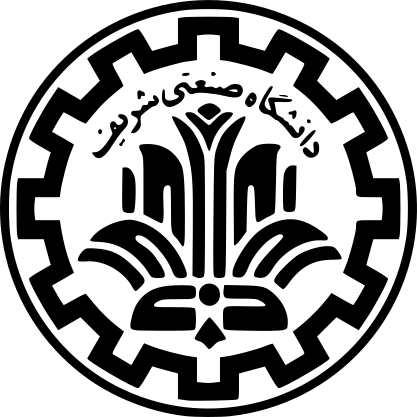
\includegraphics[width=0.5\textwidth]{logo.png}
	\end{flushleft}
	\begin{flushleft}
		دانشگاه صنعتی شریف\\
		دانشکده مهندسی برق\\
	\end{flushleft}
	
\end{minipage}
\\
\rule[0.1\baselineskip]{\textwidth}{1pt}
\begin{latin}

\section{4.5 Equivalent convex problems}
Show that the following three convex problems are equivalent. Carefully explain how the solution of each problem is obtained from the solution of the other problems. The problem data are the matrix $ A \in R^{m \times n} $ (with rows $ a^{T}_{i} $ ), the vector $ b \in R^{m} $, and the constant $ M > 0 $.

\begin{enumerate}
	\item The robust least-squares problem
	\begin{equation*}
		\min \sum_{i=1}^{m}  \phi(a^{T}_{i} x - b_{i})
	\end{equation*}
	with variable $ x \in R^{n}, $ where $ \phi : R \to R $ is defined as
	\begin{equation*}
		\phi(u) = \begin{cases}
			u^{2}  & |u| \geq M \\
			M(2|u|-M) & |u|<M
		\end{cases}
	\end{equation*}
	(This function is known as the Huber penalty function; see §6.1.2.)
	\item
	The least-squares problem with variable weights
	\begin{gather*}
		\min \sum_{i=1}^{m} (a_{i}^{T}x - b_{i})^{2}/(w_{i}+1) + M^{2} 1^{T} w
		\\
		\text{subject to : } w \succeq 0
	\end{gather*}
	with variables $ x \in R^{n} $ and $ w \in R^{m}$, and domain $ D = \{(x, w) \in R^{n} \times R^{m} | w \succ -1\}. $
	\\
	Hint. Optimize over $ w $ assuming $ x $ is fixed, to establish a relation with the problem in part (a).
	\\
	(This problem can be interpreted as a weighted least-squares problem in which we are allowed to adjust the weight of the $ i $th residual. The weight is one if $ w_{i} = 0 $, and
	decreases if we increase $ w_{i} $. The second term in the objective penalizes large values of $ w $, i.e., large adjustments of the weights.)
	\item The quadratic program
	\begin{gather*}
		\min \sum_{i=1}^{m} (u^{2}_{i} + 2Mv_{i})
		\\
		\text{subject to : } -u - v \preceq Ax - b \preceq u + v
		\\
		0 \preceq u \preceq M1
		\\
		v \succeq 0.
	\end{gather*}
\end{enumerate}
\textcolor{red}{\textbf{Solution:}}
\\
For showing this equivalency, we only need to show problem (1,2) and (1,3) are equal.  
\\
\begin{itemize}
	\item problem (1,2)
\begin{gather*}
	f(z,w) = \frac{z^{2}}{1+w} + M^{2}w \Rightarrow \dfrac{\partial}{\partial w} f(z,w) = 0 
	\\
	\Rightarrow - \frac{z^{2}}{(1+w)^{2}} + M^{2} = 0 \Rightarrow w^{*} = \frac{|z|}{M} - 1
\end{gather*}
if $ w^{*} = \frac{|z|}{M} - 1 > 0 $, this $ w^{*} $ is optimum. Otherwise, we should consider $ w^{*} = 0 $. 
\\
By taking $ z = a_{i}^{T}x - b_{i} $, we will have 
\begin{equation*}
	w^{*} = \max (0, \frac{|a_{i}^{T}x - b_{i}|}{M} - 1)
\end{equation*}
So the second problem reduce to
\begin{equation*}
	\min \frac{(a_{i}^{T}x - b_{i})^{2}}{1+w} + M^{2}w = \begin{cases}
		M(2|a_{i}^{T}x - b_{i}|-M)  & |a_{i}^{T}x - b_{i}| \geq M 
		\\
		(a_{i}^{T}x - b_{i})^{2} & o.w
	\end{cases}
\end{equation*}
By summation over $ i $, we will see the first problem.
\item problem (1,3)
we first should understand the relation between $ v $ and $ u $. For all $ i $, we should have $ v_{i} + u_{i} = |a_{i}^{T}x+b_{i}|$.
If not: 
\begin{enumerate}
	\item $ v_{i} + u_{i} > |a_{i}^{T}x+b_{i}| $. By reducing $ v_{i} $ or $ u_{i} $, we can reduce the objective function. This can be done because $ v_{i} $ and $ u_{i} $ can not be both zero. (Because $ |a_{i}^{T}x+b_{i}| \geq 0$ )
	\item $ v_{i} + u_{i} < |a_{i}^{T}x+b_{i}| $. Because of the first constrain, $ a_{i}^{T}x+b_{i} \leq 0$. So this will say that $ - v_{i} - u_{i} > a_{i}^{T}x+b_{i} $ which is against the first constrain. 
\end{enumerate}
So we will have $ v_{i} = |a^{T}_{i} x - b_{i}| - u_{i} $
\begin{gather*}
	\min \sum_{i=1}^{m}(u^{2}_{i} - 2Mu_{i} + 2M|a^{T}_{i} x - b_{i}|)
	\\
	\text{subject to : } 0 \leq u_{i} \leq \min \{M, |a^{T}_{i}x- b_{i}|\}
\end{gather*}
If $ M < |a^{T}_{i}x- b_{i}| $, so $  0 \leq u_{i} \leq M $. Then the best option for $ u_{i} $ is $ M $ and the $ i $th term of objective function will be 
$ 2M|a^{T}_{i} x - b_{i}|-M^{2} $.
Otherwise if $ M > |a^{T}_{i}x- b_{i}| $, so $  0 \leq u_{i} \leq |a^{T}_{i}x- b_{i}| $. Then the best option for $ u_{i} $ is $ |a^{T}_{i}x- b_{i}| $ and the $ i $th term of objective function will be $|a^{T}_{i} x - b_{i}|^{2}$.
So the third problem is equal to the first one.
\end{itemize}

\end{latin}